\subsection{Variador- PLC}
\subsubsection{Cable de comunicación DB9 - RS485}
Para poder realizar la comunicación entre el variador y el PLC es necesario contar con un cable que realice la conexión desde la salida CANOpen a RS485. Se necesitó hacer la construcción de dicho cable con las fichas correspondientes siguiendo las conexiones que muestran en la Figura \ref{fig:cable}

\begin{figure}[htbp]
    \centering
    \subfigure[Ficha entrada variador]{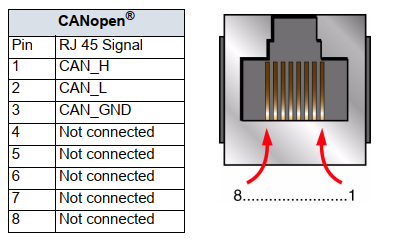
\includegraphics[width=60mm]{canconectores.png}}
    \subfigure[Ficha entrada PLC]{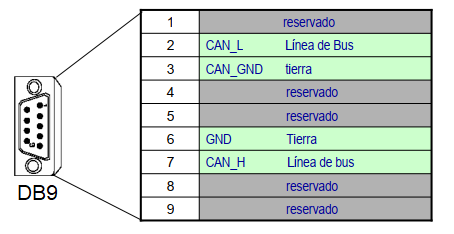
\includegraphics[width=80mm]{candb9.png}}
    \caption{Conexión fichas RJ45- DB9} \label{fig:cable}
    \end{figure}

\subsection{Motor-Variador- PLC}
\subsection{Visualización de registros}